\chapter{Introduction}
\label{chap:introduction}

% [ALL CHAPTERS] Start with sentences that tell the reader what the chapter will contain.
% What is the task + figure
%% Toy/simplified examples are often useful here
% What is the motivation and why its important
% Challenges
%% Existing approaches and their limitations
% Your approach + figure (to motivate your approach)
% List of contributions
% Thesis outline
% [ALL CHAPTERS] End with a sentence or two that links to the next chapter

\section{The need for optimisation}
\label{sec:optimisation_need}

Optimisation is everywhere. In nature, physical systems self-organise towards a state of minimum energy. Proteins have complex structures that maximise their stability and function. Light rays travel in the most efficient path to their destination. In society, businesses strive to maximise users and profit. City planning is optimised for the flow of traffic. Engineering processes aim to maximise efficiency and minimise waste.

Optimisation is paramount in the performance of many real-world systems and models. Within the last decade, optimisation has been key in enabling the deep learning revolution in the field of machine learning (ML). This has resulted in state-of-the-art (SOTA) performance in tasks such as ImageNet for image classification \citep{imagenet} and AlphaFold for protein folding prediction \citep{alphafold}. Recently, with advances in hardware, large language models (LLM) have been able to offer agentic experiences that enable human-like interactions. 

For these models to perform well, they need to learn complex concepts from a set of data and be able to generalise. The process of navigating the model to do this is the role of optimisation in deep learning. Given some \textit{objective}, a quantitative measure of the model's performance, that is dependent on a set of \textit{parameters}, the optimisation process is finding the right parameters that optimises the objective. For example, the objective for protein folding prediction could be to find a minimum energy conformation and the parameters could be the positions of the atoms of proteins and their orientations. 

Throughout the years, many optimisation algorithms have been proposed for deep learning. At the most fundamental level, these can be categorised into either first-order or higher-order methods. First-order methods guide the model by using information obtained from the \textit{first derivative} of the objective. High-order methods use information from the \textit{second derivative} onwards. Currently widely adopted and SOTA optimisers, such as SGD \citep{robbins1951stochastic} and Adam \citep{kingma2014adam}, are based on first-order methods due to computational efficiency, scalability, and good generalisation. 

\section{The curse of dimensionality and saddle points}
\label{sec:curse_of_dimensionality}

However, the process of optimisation becomes increasingly difficult as the number of parameters increase. More specifically, the landscape of our models becomes very complex as we scale with dimensionality. An example is shown in \cref{fig:high_dim_resnet}. In these high-dimensional spaces, we see a phenomenon where there is exponentially more frequent \textit{saddle points} than the points that optimise our objective \citep{dauphin2014sfn}. 

\begin{figure}[h]
  \centering
    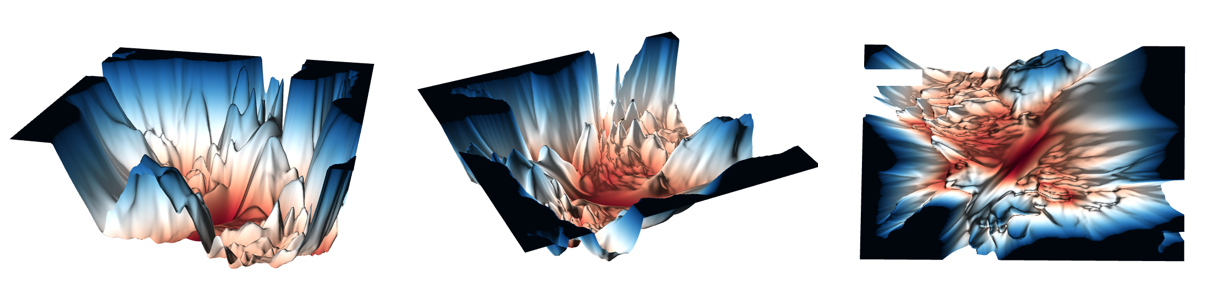
\includegraphics[width=\textwidth]{figures/0intro/intro_landscape.png}
    \caption{A visualisation of the loss landscape of a ResNet-56 model for image classification.}
    \label{fig:high_dim_resnet}
\end{figure}

A saddle point is where among some dimensions, the second-order derivative of the objective is negative, but along others, it is positive. First-order methods slow down in saddle points since they perceive it as a flat region and do not have information about the curvature of the surrounding landscape. This hinders their convergence to a good solution. 

Higher-order methods, by incorporating this curvature information, can identify the nature of saddle points and navigate away from them more effectively. Despite this, it becomes computationally infeasible to process higher-order information. This is because to obtain higher-order information, we would require at least $O(N^2)$ space for $N$ parameters. The computational cost of obtaining higher-order information becomes prohibitive as $N$ increases, which is the case given our deep learning setting. As a practical example, a ResNet-50 model has $N = 25 \times 10^6$ parameters. If we consider each parameter to be represented by 16-bits, we would require $1.25 \times 10^{15}$ bytes, or $1.25$ terabytes of memory to store the second-order information. This is in stark contrast to the $25$ million bytes, or $25$ megabytes, required for first-order information.

\section{KryBall: the best of both worlds}
\label{sec:kryball_intro}

The challenge is to therefore develop an optimisation algorithm that is computationally tractable and scalable, like first-order methods, but can also navigate complex loss landscapes, particularly by escaping saddle points, like higher-order methods. In this thesis, we propose a new optimisation algorithm, KryBall, that combines the benefits of first-order and higher-order methods. We summarise our approach below.

\begin{enumerate}
  \item We use a \textit{Krylov subspace} to approximate local curvature information as a low-dimensional subspace via efficient Hessian-vector products (HvPs).
  \item We analyse this subspace to understand the dominant geometric features of the local landscape. 
  \item We compute the \textit{Saddle-Free Newton} (SFN) direction as a result \citep{dauphin2014sfn}.
  \item We combine this with first-order information such as the gradient and momentum in a \textit{trust region} framework that uses a quadratic model approximation of the local landscape to get a combined, final search direction.
  \item We perform the optimisation step with this direction to optimise our objective.
  \item Optionally, we embed KryBall as a hybrid approach with first-order optimisers such as SGD and Adam, allowing it to be cycled through.
\end{enumerate}

KryBall makes more informed steps than pure first-order methods, particularly in regions like saddle points, while remaining computationally tractable for deep learning. To motivate our method, we show an example in \cref{fig:toy_example}, where first-order methods such as Adam and SGD are hindered on a classic 2D horse saddle, but KryBall successfully escapes it quickly in fewer iterations.

\textbf{TODO: Make into subfigures.}

\begin{figure}[h]
  \centering
    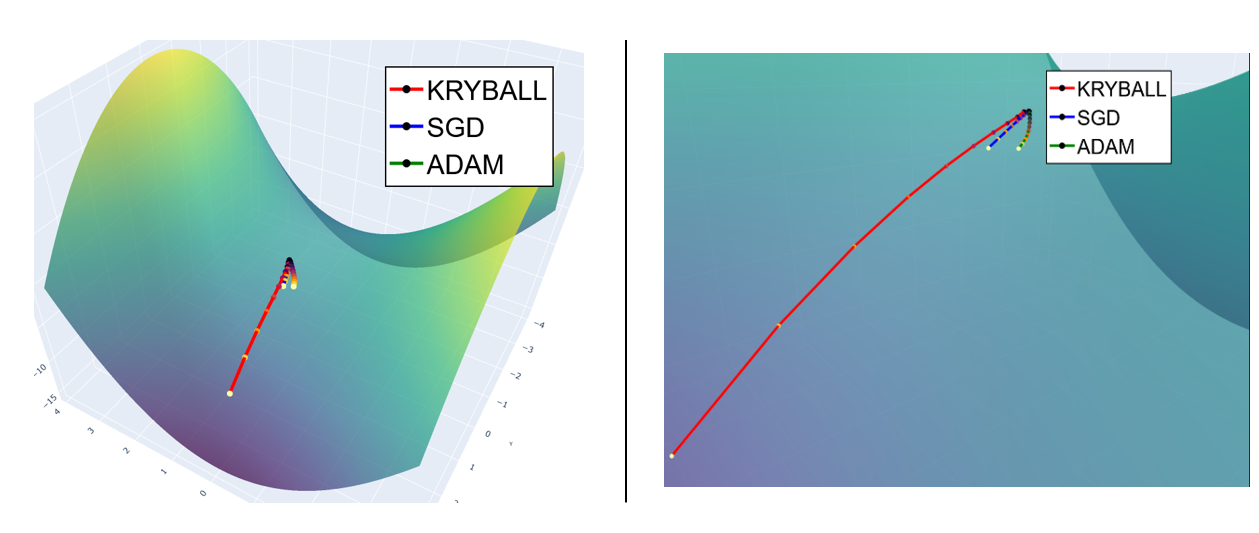
\includegraphics[width=0.85\textwidth]{figures/0intro/intro_toy.png}
    \caption{Left: A classic 2D horse saddle with KryBall, SGD and Adam. Right: A zoomed in version. KryBall successfully escapes the saddle point.}
    \label{fig:toy_example}
\end{figure}

\section{Contributions}
\label{sec:contributions}

Our work focuses on the design and implementation of a novel optimisation algorithm for deep learning, KryBall. In this thesis, we present:
\begin{enumerate}
    \item \textbf{The KryBall Optimisation Algorithm:} The proposal, design, and implementation of KryBall. We combine the benefits of first-order and higher-order methods. KryBall leverages Krylov subspace methods and the SFN direction in a trust-region framework. This enables efficient approximation of local curvature information and navigation of complex loss landscapes, while remaining computationally tractable.
    \item \textbf{Analysis of Loss Landscape Characteristics:} An analysis of the loss landscape properties of common deep learning models and the result of architectural choices (such as activation functions). We investigate the assumptions made when designing an optimiser and the impact of these assumptions on the optimisation process.
    \item \textbf{Extensive Empirical Evaluation:} Experimental validation of KryBall across a range of tasks, such as function optimisation, image classification, and image reconstruction. 
    (\color{red}{can also add the interpretability work here if needs to be more diverse.}\color{black}).
    \item \textbf{A Flexible Experimental Suite:} The development of a modular and configurable software framework for optimiser experiments. This provides a flexible and extensible framework for the implementation, testing, and comparative analysis of various optimisation algorithms. 
    (\color{red}{while not research --- I do think the current framework is a good software suite for a range of tasks that I haven't seen much for optimiser research (except MLPerf). It's quite easy to use, efficient, and extensible. Happy to remove if it doesn't really count as a contribution.}\color{black}).
\end{enumerate}

\section{Thesis outline}
\label{sec:thesis_outline}

To present our contributions, this thesis is organised in the following manner:

\begin{itemize}
    \item \cref{chap:background} provides a mathematical background on optimisation. We formalise the optimisation problem and discuss the geometry of optimisation, including saddle points. This is followed by optimisation in deep learning, where first-order and higher-order methods are explained. We then introduce Krylov subspace methods and trust region algorithms.
    \item \cref{chap:lit_review} provides a comprehensive review of the relevant literature. This includes a survey of first-order and higher-order optimisation algorithms used in deep learning. We compare these methods with our own.
    \item \cref{chap:method} presents the KryBall algorithm. We formally describe its components. This includes the Krylov subspace construction, the SFN computation, and integration with the trust-region framework. We also discuss the assumptions made during the design and outline the hybrid approach.
    \item \cref{chap:results} presents our evaluations. We describe our experimental setup and benchmarking suite. This includes the datasets, model architectures, evaluation metrics, hyperparameter configurations, and comparison with SOTA optimisers. We then present sensitivity analysis and ablation studies.
    \item \cref{chap:discussion} discusses the results. We interpret our findings, analyse potential failure cases and unexpected behaviours, and address current limitations. 
    \item \cref{chap:conclusion} finishes the thesis. We summarise our contributions, discuss the implications of our work, and suggest future work.
\end{itemize}

This chapter has laid the outline for the thesis. We now proceed to \cref{chap:background} to establish the necessary mathematical context.